%\documentclass[conference]{IEEEtran}
\documentclass[conference]{worldcomp}

\usepackage[hmargin=15mm,vmargin=1in]{geometry}
\usepackage[american]{babel}
\usepackage[T1]{fontenc}
\usepackage{times}
\usepackage{caption}
\usepackage{textcomp}
%\usepackage{epsfig,graphicx}
\usepackage{amsfonts,amsmath,amssymb}
%\usepackage{fixltx2e} % Fixing numbering problem when using figure/table* 
\usepackage{booktabs}

\usepackage{cite, graphicx, subfigure, listings, xspace, txfonts} 

\columnsep 6mm

\title{FCNP: Fast I/O on the Blue Gene/P}


\author{John W. Romein \\[3mm]
\texttt{romein@astron.nl}\\
Stichting ASTRON (Netherlands Institute for Radio Astronomy), Dwingeloo, The Netherlands}

\newcommand{\us}{\,$\muup$s\xspace}
\newcommand{\ns}{\,ns\xspace}

\begin{document}

\maketitle

\begin{abstract}
This paper describes the \emph{Fast Collective-Network Protocol (FCNP)}.
FCNP is a low-overhead, high-bandwidth network protocol that we developed for
fast communication between the Blue Gene/P compute nodes and I/O~nodes.
The CPU cores in this system are hardly able to keep up with the high-speed
internal network, and any protocol overhead significantly slows down the
achieved bandwidths.
%To scale up from its predecessor Blue Gene/L, a Blue Gene/P I/O~node must
%communicate nearly five times faster, but the speed of a processor core was
%increased by only 21\%.
%Hence, the impact of communication overhead is increasingly profound.
FCNP minimizes overhead and approaches the link speed for large messages.

FCNP is of critical importance to the correlator of the LOFAR radio telescope,
that will process hundreds of gigabits of real-time telescope data per second.
Without FCNP, the correlator would not even achieve the required data rates.
However, FCNP allows bandwidths over 50\% beyond the LOFAR requirements,
so that the telescope can observe proportionally more sources or frequencies
and becomes a much more efficient instrument.
\end{abstract}

\vspace{1em}\noindent
\textbf{Keywords:} {\small low-overhead network protocol, IBM Blue Gene/P, LOFAR radio telescope}


\section{Introduction}

I/O is one of the most precious resources in a supercomputer~\cite{Iskra:08},
and the IBM Blue Gene is no exception to this rule.
Although the Blue Gene/P uses much faster I/O~hardware than
its predecessor Blue Gene/L, we found that it is still difficult to
efficiently stream large amounts of data from outside the system to the
final destination CPUs.
%This is partly due to the small amount of internally available I/O~hardware
%that is used for external I/O, and partly due to inefficient use of the
%hardware that is available.

The Blue Gene architecture consists of compute nodes that run a parallel
application and a much smaller number of I/O~nodes that perform
I/O operations on behalf of the compute nodes.
The I/O nodes and compute nodes are internally connected by what is called the
\emph{tree\/} or \emph{collective network}.
The system software forwards I/O operations like \texttt{read()} and
\texttt{socket()} from a compute node to its associated I/O~node where the
operation is factually performed.

By default, the I/O~nodes work transparently.
However, the performance of I/O-intensive applications can improve
significantly if a select part of the application or communication library
(like PVFS) runs on I/O~nodes rather than compute nodes~\cite{Iskra:08}.

We use the Blue Gene to process real-time radio-telescope data.
Part of the application runs on the I/O~nodes, while the compute-intensive
processing is done on compute nodes.
The application on the I/O~node needs to communicate large amounts of data
with the application on the compute nodes.

In 2007, IBM unveiled the Blue Gene/P (BG/P)~\cite{IBM:08} as successor to
the Blue Gene/L (BG/L).
Per rack, the BG/P has 2.43 times as much compute power as the BG/L.
However, the (maximum) number of I/O~nodes per rack has \emph{halved}, due to
the change from 1~to 10~Gb/s Ethernet technology.
Hence, to scale with the computational performance, each I/O~node has to
handle 4.86 times as much data.
This is challenging, since the tree is only 2.43~times faster.
However, the main challenge is that the processor cores that drive the tree
are merely \emph{21\%\/} faster.
Fortunately, the I/O nodes have four cores rather than two, but at most two
cores can be used for internal communication: one to read and one to write the
tree.
The remaining cores can be used for other tasks.

We found that a core is hardly able to read or write packets at
link speed from or to the tree; even an ``empty'' function call per packet
already ruins performance.
The overhead of any protocol on top of the packet interface would decrease
the obtained bandwidth significantly.

%Even worse: data that are received via the 10~Gb/s Ethernet interface of an
%I/O~node can only be forwarded over a much \emph{slower\/} (6.8~Gb/s)
%internal link to the compute nodes.

This paper describes the \emph{Fast Collective Network Protocol\/} (FCNP),
that is designed to provide bandwidths at link speed between the I/O~nodes
and the compute nodes.
The key design feature of FCNP is that it maximizes bandwidth by minimizing
protocol overhead to an absolute minimum.
By reducing the protocol overhead, the processor cores have more time to
transport user data.
We will show performance results and characterize the performance in terms
of bandwidth, latency, and overhead.

\addtocounter{figure}{1}
\begin{figure*}[t]
\includegraphics[width=\textwidth]{processing.pdf}
\caption{LOFAR real-time signal processing.}
\label{fig:processing}
\end{figure*}

FCNP is heavily used to process LOFAR telescope data.
LOFAR~\cite{Butcher:04,deVos:09} is the first of a new generation of
telescopes, that
combines the signals of tens of thousands of simple, cheap, omni-directional
antennas rather than using expensive dishes.
In several ways, it will be the largest telescope of the world.
Another novel feature is that the data are processed in \emph{software\/} on a
supercomputer~\cite{Romein:06,Romein:09b}, where traditionally custom-built hardware is
used.
The data are streamed at high bandwidths into the system and processed in real
time.
I/O~nodes receive the data and internally forward them to compute nodes.
Standard system software does not provide sufficient bandwidth to handle
2.1~Gb/s input and 0.58~Gb/s output per I/O~node, needed to meet the LOFAR
specifications~\cite{LOFAR_SPECS}.
In contrast, FCNP achieves 3.1~Gb/s input and 1.2~Gb/s output bandwidth per
I/O~node.
The improved input data rate matches the absolute maximum that the telescope
hardware can generate, which is \emph{over 50\% beyond\/} the specifications.
This implies that LOFAR will be able to observe a 50\%~wider part of the radio
spectrum instantaneously, or to observe 50\%~more sky sources concurrently,
increasing the usage possibilities of the instrument.
The doubled output data rate allows new observation modes, where even higher
numbers of sky sources can be observed concurrently (albeit at lower
precision), increasing the flexibility of the instrument.

We developed FCNP to support streaming LOFAR data,
but the ideas of this protocol are more widely applicable.

This paper is structured as follows.
In Section~\ref{sec:LOFAR}, we describe the relevant parts of the LOFAR
processing pipeline.
Then, after an introduction to the BG/P
hardware (Section~\ref{sec:BG/P}), we describe FCNP (Section~\ref{sec:FCNP}).
Next, we discuss related work (Section~\ref{sec:related-work}).
We compare the performance of FCNP to competing protocols and analyze the
performance impact on the LOFAR application (Section~\ref{sec:performance}).
Section~\ref{sec:conclusions} concludes.



\section{LOFAR processing}
\label{sec:LOFAR}

LOFAR is a new type of radio telescope, that combines the signals of tens of
thousands of antennas and processes the data centrally on a BG/P supercomputer.
We briefly explain how LOFAR data are processed, other papers provide more
details~\cite[Sec.~2]{Romein:06},~\cite[Sec.~4--6]{Romein:09b}.

\addtocounter{figure}{-2}
\begin{figure}[h]
\begin{center}
\includegraphics[width=.7\columnwidth]{station.jpg}
\end{center}
\caption{The low-band antennas of a LOFAR station.}
\label{fig:station}
\end{figure}
\addtocounter{figure}{1}

Co-located groups of 48 or 96 dual-polarized low-band antennas (see
Figure~\ref{fig:station}) and high-band receivers form a \emph{station},
i.e.\ a virtual telescope.
Construction of 36--54 Dutch stations and 8--20~European stations is well
underway.
Each station digitizes the antenna voltages and pre-processes the data using
FPGAs~\cite{Gunst:07}.
The FPGAs send UDP packets with station data over dedicated Wide-Area
Network links to the BG/P, where the data are centrally processed.
Initially, LOFAR used a 6-rack IBM BG/L supercomputer for real-time
processing of the station data, but the system was recently replaced by an
equally powerful 2.5-rack BG/P.

The application that runs on the BG/P is called the \emph{correlator},
although it does much more processing than correlating only.
Figure~\ref{fig:processing} shows a simplified scheme of one of the processing
pipelines: the standard imaging pipeline that creates sky images.
An I/O~node receives 48,828 UDP packets per second of up to 8\,KiB from one
station.
It copies the samples into a circular buffer that holds the most recent
three seconds of data.
The buffer is used to synchronize the stations (the travel times over the
WAN are higher for remote stations than for nearby stations) and to prevent
data loss due to small hiccups in the remainder of the processing pipeline.
The buffer is also used to set the observation direction by ``delaying''
the stream of station samples for each station differently, to compensate for
the fact that a celestial wave hits stations at different
times~\cite[Sec.~2.1]{Romein:06}.

The buffered data are sent to the compute nodes for further processing.
There, the data are first exchanged over the torus network, to collect pieces
of data that can be processed independently.
Then, the data are filtered and Fourier transformed to split each subband into
narrow frequency channels.
Next, a phase correction fine-tunes the observation direction.
Then, a per-channel bandpass correction flattens a ripple introduced by
a station filter.
Optionally, a group of stations can be beam formed (by weighted addition of
their samples) to form a more sensitive, virtual ``super station''.
Finally, the data are correlated (by multiplying the samples of all station
pairs) to filter out noise and integrated to reduce the amount of output.

The compute node sends the correlated data back to the I/O~node.
The I/O node optionally adds data from other compute nodes, and sends the
result (asynchronously) to external systems that temporarily store the data
on disk.
After an observation has finished (not shown in Figure~\ref{fig:processing}),
bad data (due to interference) are removed, and the
resulting data are calibrated~\cite{Nijboer:07} and imaged.

Two tasks are of particular interest to this paper: the transport of buffered
data from the I/O~nodes to the compute nodes (at 3.1~Gb/s) and the transport
of correlated data in the opposite direction (at up to 1.2~Gb/s).
Moreover, each I/O~node also needs to receive 3.1~Gb/s of UDP data from the
stations and send 1.2~Gb/s of TCP data to external systems, and are therefore
already quite busy processing the data through the IP protocol stack.
The two available mechanisms to communicate between the
I/O~nodes and compute nodes (TCP and Unix domain sockets) do not provide
sufficient bandwidth (see Section~\ref{sec:performance}) and consume
too many CPU resources,
necessitating the need for a light-weight protocol for internal communication.


\section{The Blue Gene/P}
\label{sec:BG/P}

%Below, we describe the key features of the Blue Gene/P.

%This system contains 10,880 cores that provide 37.0~TFLOPS peak processing
%power.

The BG/P is built using SoC (System-on-a-Chip) technology that integrates
all processing and networking functionality on a single die.
A node contains four PowerPC~450 cores, running at a modest 850~MHz clock
speed to reduce power consumption and to increase the package density.
Each core is extended by two Floating-Point Units that provide support for
operations on complex numbers; each FPU can sustain one (real) double-precision,
fused multiply-add per cycle.
The four cores share 2~GiB of main memory.
One BG/P rack contains 1,024 compute nodes, providing 13.9~TFLOP/s peak
processing power, and up to 64 I/O~nodes.

The BG/P contains several networks.
A fast \emph{three-dimensional torus\/} connects all compute nodes and is used
for point-to-point and all-to-all communications.
The \emph{tree\/} or \emph{collective network\/} is used for MPI scatter and
gather operations, but also for communication between compute nodes and
I/O~nodes.
A \emph{10~Gb/s Ethernet device\/} (only enabled on I/O~nodes) is used for
external communication.
A \emph{global interrupt network\/} provides support for fast barriers.
Additional networks exist for initialization, diagnostics, and debugging.

%We typically run our application in \emph{virtual node mode}, where the
%the processor and memory are logically split into four independent nodes.
%Compared to \emph{SMP mode}, this simplifies programming, since this allows
%single-threaded processing on the compute nodes.
The compute nodes run a fast, simple kernel (Compute Node Kernel, CNK) that
can execute one thread or process per core.
An I/O~node uses the same hardware as a compute node, but runs a modified
Linux kernel.


\subsection{The Tree Network}

\begin{figure}[h]
\includegraphics[width=\columnwidth]{pset.pdf}
\caption{A pset.}
\label{fig:pset}
\end{figure}

Each compute node is (indirectly) connected to one I/O~node via the tree
(see Figure~\ref{fig:pset}).
All I/O-related system calls on the compute nodes to external systems are
forwarded to a daemon program (CIOD), that runs on the
I/O~node and performs the real operation.
A group of one I/O~node, its 10~Gb/s Ethernet interface, and the compute
nodes that are connected to the I/O~node is called a \emph{pset}.
Since LOFAR generates much data, our system is configured with
the maximum number of 1~I/O~node per 16~compute nodes (64~cores); typical
installations have 1~I/O~node per 32~compute nodes.
Our system has 160~psets in total.

The original BG/L design did not support the idea of running user applications
on the I/O~nodes, but in earlier work~\cite{Iskra:08}, we showed that doing so 
significantly improved performance, flexibility, and costs.
Unfortunately, this required major changes to the BG/L system
software~\cite{Iskra:08,Boonstoppel:08}.
In contrast, the BG/P supports user applications on I/O~nodes, but
the existing communication protocols between the compute nodes and the
I/O~nodes provided insufficient bandwidth for the LOFAR correlator.

The tree uses bi-directional links at 6.8~Gb/s per direction.
The network has a tree topology with a complex physical structure.
A node is connected to at most three other nodes.
A packet can be routed via several nodes.
The processor cores of in-between nodes are not interrupted by the routing
process.
The hardware provides two separate virtual channels.
One is used by CIOD;
the other is typically only used on the compute nodes: by the MPI library for
some of the collective MPI operations.
However, the runtime environment can be changed so that MPI uses the
3-D~torus for these collectives instead of the tree, leaving one of the virtual
channels unused.
This virtual channel is accessible from user space.

The LOFAR correlator does not perform collective MPI operations.
However, other applications that critically depend on collectives might
see performance differences (positive or negative) by using the 3-D torus
instead of the tree.
On the BG/L, the collective network was specifically designed to
support collective operations.
However, the BG/P is very well capable of doing collective operations
using the torus, since the BG/P has DMA support for the torus
(but not for the tree).
Therefore, FCNP can use the free virtual channel, without significantly
slowing down collective operations.

A processor can send and receive fixed-size packets over a virtual channel.
A packet consists of a 4-byte header (used for routing) and 256 bytes payload.
The 16-byte load and store instructions from the double FPU are used to
efficiently transfer data from memory to the (memory-mapped) device and vice
versa, but these impose a 16-byte alignment restriction.
There is no DMA hardware available for the tree.
The four cores from one processor share the same link.
Each node has an 8-packet send FIFO and an 8-packet receive FIFO per virtual
channel.
An attempt to send a packet to a processor with a full receive FIFO blocks
the virtual channel, filling up the sender's send FIFO, and eventually stopping
the sender.
Therefore, received packets should be consumed as fast as possible.

%The tree network (at 6.8~Gb/s) is slower than the 10~Gb/s Ethernet device.
%However, faster links between the I/O~node and the compute nodes would not
%have increased the bandwidth between the compute nodes and external systems,
%since the cores at the I/O~nodes can process only roughly 6~Gb/s through
%the TCP/IP stack.
%Forwarding the data over the tree reduces this bandwidth to XXX~Gb/s, and
%is fully limited by the CPU speed.


\section{The Fast Collective Network Protocol}
\label{sec:FCNP}

CIOD (the daemon that runs on the I/O~node and handles the I/O~requests from
the compute nodes) is intended to provide communication between compute nodes
and external systems.
It is also possible to use TCP or Unix domain sockets internally,
between an application on the compute nodes and an application on the I/O~node.
However, the obtained bandwidth (see Section~\ref{sec:performance}) is
insufficient for the LOFAR correlator.
Therefore, we developed a new protocol, \emph{Fast Collective Network
Protocol\/} (FCNP), that uses the free virtual channel of the tree.

Since one compute core is barely able to keep up with the link speed,
any heavy-weight protocol overhead would decrease the obtained bandwidth.
FCNP reduces the protocol overhead to a single bit test in the normal case.
FCNP distinguishes control packets (requests and acknowledgments) from data
packets by setting the Irq (interrupt-on-receipt) bit in the header.
Typically, most packets (for our application roughly 99.98\%) are data packets
that do not contain any metadata in the payload part.

\begin{figure}[h]
\subfigure[write.]{
  \includegraphics[width=.46\columnwidth,height=35mm]{FCNP-write.pdf}
  \label{fig:FCNP-write}
}
\hfill
\subfigure[read.]{
  \includegraphics[width=.46\columnwidth,height=35mm]{FCNP-read.pdf}
  \label{fig:FCNP-read}
}
\caption{The FCNP protocol.}
\label{fig:FCNP-protocol}
\end{figure}

To send data from the compute node to the I/O~node, the application on the
compute node calls \emph{fcnp\_write(ptr, size)\/} and the application on the
I/O~node calls \emph{fcnp\_read(ptr, size, core)}.
The compute node sends a write request packet to the I/O~node~(see
Figure~\ref{fig:FCNP-write}).
The I/O~node acknowledges a write request as soon as the application called a
matching \emph{fcnp\_read()} for that particular core \emph{and\/} when no
other compute node is sending data to this I/O~node.
This way, the I/O~node knows at all times from which compute core data packets
originate, and can receive data packets consecutively in memory without
additional checks.
Only the Irq bit must be checked to see if the packet is indeed an expected
data packet, and not a request packet from another compute core.
The actual amount of bytes sent in a message is negotiated by the compute node
and the I/O~node by taking the minimum of the requested sizes on both sides.
A read request (see Figure~\ref{fig:FCNP-read}) is handled similarly.
At any time, up to one read and one write per pset can be active (although
multiple unacknowledged request can be outstanding).

\begin{figure}[h]
\lstset{language=C,basicstyle={\fontencoding{T1}\fontfamily{pcr}\fontseries{m}\fontshape{n}\fontsize{8}{10pt}\selectfont}}
\begin{lstlisting}{}
struct RequestReplyPacket {
  enum {READ, WRITE, RESET} type;
  unsigned                  node;
  unsigned short            core;
  unsigned short            rankInPSet;
  unsigned                  size;
  char                      msgHead[240];
};
\end{lstlisting}
\caption{Format of the payload part of request and acknowledgment packets.}
\label{fig:control-packet-format}
\end{figure}

Figure~\ref{fig:control-packet-format} shows the format of request and reply
packets.
A request is a \emph{read}, \emph{write}, or a \emph{reset\/} packet
(reset requests are only sent during startup, to drain the FIFOs that may hold
lingering packets from previous runs).
The \emph{node}, \emph{core}, and \emph{rankInPset} fields are the node number,
the compute core number (between 0~and~3), and the rank within the pset
respectively.
These are necessary for the I/O~node to determine the source of a request
and to put routing information in the header of a reply.
The \emph{size} field in a request contains the requested message size;
the \emph{size} field in an acknowledgment contains the agreed size, which
may be smaller than the requested size if the I/O-node application does not
want to read or write as much data.
The last 240~bytes of a read acknowledgment or a write request are used to
send up to 240 bytes of data, such that the remaining amount of data is a
multiple of 256 bytes, and can be sent in an integer number of packets.

To avoid deadlocks, it is always a \emph{compute core\/} that initiates
communication by sending a (read or write) request packet to the I/O~node.
Compute nodes are not always willing or able to receive data, and
if the I/O~node would send a packet to a compute node that does not listen,
the tree could block.
The I/O~node, in contrast, runs a daemon thread that continuously polls the
receive FIFO, waiting for an incoming request packet.
This way, the tree cannot stall.
The polling thread is suspended while another thread receives data packets
from a compute node.

Each of the four cores in a compute node can post a read or write request.
To avoid race conditions, only one of them is allowed to read the receive FIFO.
As long as none of the request is acknowledged, one of the cores that await
a reply polls the FIFO until it receives an acknowledgment.
If the acknowledgment is addressed to another core, it transfers the packet
(via shared memory) to the other core and releases its access rights.
A compute core that receives a read acknowledgment gains exclusive access to
the receive FIFO until the message is completely received.
The sequence of data packets might be interrupted by a write acknowledgment
for another core, which is then transferred to the addressed core.
This interruption is detected by testing the Irq bit in the header.
The stream cannot be interrupted by a read acknowledgment, since the I/O~node
makes sure that only one read can be active at a given time.
%Transferring ownership of the receive FIFO is complicated and prone to
%race conditions.

On the compute cores, we use fast hardware mutexes to synchronize the cores.
On the I/O~nodes, the same hardware mutexes are physically present, but not
exposed by the Linux kernel, so we use atomic instructions to implement spin
locks.
Since these are noticeably slower and since the write FIFO has to be protected,
the implementation writes up to eight consecutive packets before releasing
and re-obtaining a lock.
This way, the amortized locking overhead is negligible.

FCNP strongly encourages 16-byte aligned data and message sizes, but
does not enforce this.
Unaligned transfers are supported at the expense of a copy to an
intermediate buffer.

\begin{figure}[h]
\begin{center}
\begin{vbox}
\subfigure[Unshared bandwidth.]{
  \includegraphics[width=\columnwidth]{unfair.pdf}
  \label{fig:unfair}
}
\end{vbox}
\vspace{5mm}
\subfigure[Shared bandwidth.]{
  \includegraphics[width=\columnwidth]{fair.pdf}
  \label{fig:fair}
}
\end{center}
\caption{Unfair communication is faster (see text).}
\label{fig:fair-unfair}
\end{figure}

FCNP is not fair, in the sense that one core can claim all network bandwidth.
This is intentional, since sharing bandwidth between multiple cores implies
that all cores proceed at reduced speed.
Figure~\ref{fig:fair-unfair} illustrates this with an example, where all
CPUs concurrently start communicating the same amount of data (the red, fat
bars; blue, dashed lines represent waiting CPUs).
If the bandwidth is not shared (Figure~\ref{fig:unfair}), some CPUs finish
much earlier than others, and can continue doing other work.
Even the latest CPU does not finish later than in the shared case
(Figure~\ref{fig:fair}), where all CPUs finish approximately at the same time.
In general, fairness is an issue for interactive applications and multiple
applications run by different users, but FCNP is designed to support a single,
cooperative, distributed application, of which we want to minimize the
execution time.


\subsection{Interrupts}
\label{sec:interrupts}

The polling thread on the I/O node consumes a lot of CPU resources: even if it
does not receive any data, one out of four cores is continuously busy.
A second core is fully used by CIOD to poll the other virtual channel of the
tree, leaving few resources for application processing.
To reduce the CPU usage, IBM modified the Linux device driver of the tree to
handle interrupts from both virtual channels, and adapted CIOD to take
advantage of the interrupts.
Likewise, we adapted FCNP's polling thread to block until a request packet
(with the Irq bit set) is received in the receive FIFO.

An interrupt from the receive FIFO does not necessarily imply that it is the
\emph{first\/} packet in the queue that has the Irq bit set, nor that the
packet is still in the FIFO (it might have been read before the interrupt is
processed), so care must be taken to avoid race conditions and handle spurious
interrupts.
The device driver does not use (posix-style) signals to pass on an interrupt
to an application.
Instead, a thread can do a dummy read() system call on the device driver's
file descriptor, and is blocked as long as there are no packets in the
receive FIFO that have the Irq bit set.
%A successful read() implies that there is at least one packet with the Irq
%bit set in the receive FIFO (unless another thread has already read it away).
We think that this is a much more elegant solution, since signal handlers and
threads do not coexist well.
Moreover, an implementation based on signal handlers would need to perform
additional system calls to avoid potential race conditions, thus the dummy-read
mechanism is also more efficient.

The application can choose whether FCNP should use interrupts or not.
In interrupt mode, the thread that handles new requests does not immediately
suspend itself, but polls the receive FIFO for up to 50\us.
Since applications often send multiple messages in bursts,
it is generally beneficial to try to receive a next request by polling,
to avoid the interrupt overhead~\cite{Langendoen:96}.
This significantly reduces the latency if a message arrives within 50\us,
but hardly wastes CPU resources if no message arrives within this time.

On the compute node, there is no need to interrupt the kernel (and application)
for acknowledgment packets.
Since the kernel allows only one thread per core, the core cannot be used to
run another application thread while waiting for an acknowledgment.
Only if the FCNP interface would support asynchronous reads and writes, this
would be useful, but we did not implement this, mainly because the absence of
DMA hardware would limit the use of asynchronous~I/O anyway.




%\subsection{Initialization}
%
%\emph{FIXME: deze subsectie eruit?\/}
%During the start of a program, the receive and send FIFOs can hold lingering
%packets from a previous job that crashed.
%Since data packets contain no metadata, it is not possible to distinguish
%packets from different jobs.
%To discard old packets, both the compute and I/O~nodes start reading and
%dropping packets from the receive FIFOs until it the network is completely
%drained (note that the application on the I/O~node may start earlier or later
%than the application on the compute nodes).
%Then, one core of each compute node periodically sends RESET request packets
%(some of which may be discarded by the I/O~node, until the I/O~node sends a
%RESET acknowledgment.
%After this, normal communication is possible.
%
%In the worst case, a previous program was killed half-way transmission of a
%packet, leaving the FIFO in a half-filled state.
%The FCNP library detects this during initialization of the next job.
%Half-read packets are handled by discarding the remainder of a packet.
%The current version of FCNP cannot, however, recover from half-sent packets,
%although there is hardware provision to reroute a packet that has only been
%written partially in a send FIFO.
%Since this is rather complicated, we have not yet implemented this.
%Instead, the library prints a message asking the user to reboot the partition.
%In practice, we have seen only very few occasions where a reboot was necessary.




%One reason for the low bandwidth is the fact that the collective network
%has no DMA and that the its receive FIFO must be continuously polled by
%the CPU.
%The FIFO has only 8 256-byte packet buffers and communication stalls if
%the FIFO is full.
%Another reason for the low bandwidth is the relatively low speed of the
%PowerPC core: we found that it is too slow to handle both the GbE device
%and the collective network at gigabit speed.
%Since the processor in the I/O~node is the same ASIC as those of the compute
%nodes, there is a second PowerPC core available.
%The second core is not used because the L1 caches of both caches are not
%coherent, and neither the Linux OS, nor the c and pthreads libraries can
%handle incoherent memory.
%However, with so much pressure on the first core, it was tempting to try to
%get the second core functional, and use it as some kind of ennobled DMA engine
%to offload reads from and writes to the collective network.
%After all, 2.15~TFLOPS of unexplored compute power was idling next to
%overloaded I/O-node cores.
%This way, the second core can poll the receive FIFO for incoming
%packets and copy data from memory to the send FIFO, while the first core
%can push GbE packets through the IP stack, a time-consuming task.

%The Linux kernel was modified to enable the second core and with a system
%call to move a process from one core to the other~\cite{Boonstoppel:08}.
%The ZOID daemon maintains L1-cache consistency in software --- unpleasant
%to implement, but disabling the L1 cache for message buffers greatly simplified
%this tasks and has no effect on the performance, since the data has to go
%through the shared L3 cache anyway.
%The L1-cache incoherence is hidden to the application.
%Performance measurements show that the load on the first core is indeed
%significantly reduced, roughly by 30\%.
%Offloading work to the second core was necessary to achieve the for LOFAR
%required data rates.


\begin{figure*}[t]
\subfigure[I/O~node to compute node.]{
  \includegraphics[width=.44\textwidth]{ion-to-cn-performance.pdf}
  \label{fig:ion-to-cn-performance}
}
\hfill
\subfigure[Compute node to I/O~node.]{
  \includegraphics[width=.44\textwidth]{cn-to-ion-performance.pdf}
  \label{fig:cn-to-ion-performance}
}
\caption{Measured bandwidths, as function of message size.}
\label{fig:performance}
\end{figure*}

\section{Related Work}
\label{sec:related-work}

CIOD (Control and I/O Daemon)~\cite{IBM:08} is part of the standard Blue Gene
system software and performs two major tasks: it is responsible for booting
the compute node and starting jobs (control), and for file and socket
communication from applications that run on the compute nodes.
It uses a function-forwarding mechanism to forward I/O-related system calls
from a compute node to its I/O~node, where the operations are really performed.
This function forwarding is transparent to the user.
On the BG/L, its performance was initially poor~\cite{Romein:06}, but
improved significantly later~\cite{Iskra:08}.
On the BG/P, CIOD is multi-threaded and made open source.

ZOID (ZeptoOS I/O Daemon)~\cite{Iskra:08} is a communication framework that
improves I/O performance on the Blue Gene.
ZOID is a replacement for CIOD, aimed to provide even better performance and
more flexibility.
ZOID is extensible: a small daemon on the I/O~node provides a basic function
forwarding facility from the compute nodes to the I/O~nodes.
On top of this, plug-ins (in the form of shared objects) that implement some
functionality are loaded by the daemon and perform the real work.
A standard plug-in is the \emph{Unix\/} plug-in that implements the
Unix I/O related system calls.
On the compute nodes, the glibc library was adapted to replace the Unix
system calls by stubs that forwards calls like \emph{socket()\/} and
\emph{read()}, and a shared object on the I/O~node implement the actual calls.
A stub generator creates code that marshals and unmarshals function
arguments and results on the compute nodes and I/O~nodes.

ZOID's extensibility allows arbitrary application code to be run on the
I/O~node; something that, on the BG/L, was not possible before.
Before the LOFAR BG/L was replaced by a BG/P, we used ZOID to run LOFAR-specific
application code on the I/O~nodes~\cite{Iskra:08}.

%Even though ZOID outperformed CIOD, we still did not achieve the bandwidth
%required for LOFAR on the BG/L, because the I/O node did not provide
%sufficient processing power.
%However, we recognized that each I/O node had an idling second core, unused
%because SMP Linux cannot handle incoherent L1~caches.
%To improve the ZOID performance, both the kernel and the ZOID daemon were
%modified to use the second core as coprocessor that performs two simple tasks:
%read and write the tree~\cite{Boonstoppel:08}.
%Cache coherency was maintained in software.
%This significantly decreased the load on the first core and increased the
%bandwidth beyond the required data rates.
%On the BG/P, similar techniques are not necessary, since the L1~caches
%are coherent and SMP Linux already provides access to all four cores.

ZOID was ported to the BG/P, but runs only with ZeptoOS kernels on the
compute nodes, not with the CNK.
ZeptoOS did not yet support the 3-D~torus, which is of critical
importance to the LOFAR application.
Once ZeptoOS fully supports the torus, we might use it instead of CNK.

A fundamental difference between ZOID and FCNP is that ZOID integrates system
control and application I/O into the same process.
ZOID applications (in the form of shared objects) are plugged in into the
address space of the daemon, to avoid expensive context switches during
communication.
A disadvantage of this approach is that a crashing application can crash
the control daemon as well.
Due to the availability of a free virtual channel on the BG/P,
FCNP can separate control I/O from application I/O, without performance penalty.

%A fundamental difference between ZOID and FCNP is that ZOID controls the system,
%where applications (in the form of shared objects) can be plugged into the

%A fundamental difference between ZOID and FCNP is that ZOID does system control
%and application I/O in the same process (to avoid expensive context switches),
%while FCNP is a network library that can be used by the application,
%separating control and application I/O.
%A crashing application, therefore, does not interfere with the control daemon,
%since they run as different processes.
%Separating these was only possible due to the availability of a free
%virtual channel in the collective network.
%Like ZOID, FCNP supports zero copy, provided that the data are 16-byte aligned
%(otherwise, an additional copy to temporary storage is performed).
%Fulfilling the alignment requirements, though, was unpleasant to implement.
%Unlike ZOID, the application is not a shared object that is plugged into the
%address space of the network daemon, but a normal process.
%This is somewhat simpler to use, and separates application-level~I/O from
%control and system-level~I/O.
%A crashing application does not tear down the control daemon, which runs as
%different threads in the same process in ZOID, but as separate processes in


\section{Performance}
\label{sec:performance}

Figure~\ref{fig:performance} shows the measured bandwidths for FCNP (with
interrupts enabled or disabled) and for TCP and Unix domain socket
communication using CIOD.
The benchmark communicates data between the I/O node and one of the compute
nodes as fast as possible, using messages of various sizes.
For large messages, FCNP approaches the link speed.

CIOD peaks at a bandwidth that is slightly over 2~Gb/s.
In theory, this equals the required LOFAR data rate, but we found that the
bandwidth is not stable over long times, and provides too little
headroom for real-time processing.

FCNP is significantly faster than CIOD, because its overhead is much lower.
CIOD cannot be blamed for this, since CIOD was designed to provide external,
not internal communication.
Internal communication happens to work, but a system-call interface with a
heavy-weight TCP/IP protocol is obviously less efficient.

The discontinuity in the curve for interrupt-driven FCNP in
Figure~\ref{fig:ion-to-cn-performance} is caused by the fact that the polling
thread polls the tree for 50\us after receiving a request packet, before
suspending itself (see Section~\ref{sec:interrupts}).
Messages of 64~KiB or more take over 50\us to send.
Therefore, a request for a large message causes an interrupt that increases the
latency.
In contrast, requests for smaller messages will be received through polling.
This effect is not seen in traffic from the compute node to the I/O node,
since in this direction, the 50\us timer starts running after the last
data packet was received (rather than the request packet).
Consequently, in this benchmark all subsequent requests will be received
through polling.

We use a simplified LogGP model~\cite{Alexandrov:95} to determine the
latency, bandwidth, and overhead.
We define the approximate time to send a message as the latency plus the
message size multiplied by the time to send a byte.

The latency is dominated by the receipt and handling of a request packet on the
I/O node (and would be overhead in terms of LogGP).
The latency varies depending on several circumstances.
Using the benchmark described above, the latency is 13.3\us for read
requests and 13.9\us for write requests.
We also used a different benchmark that measures the latency for the case
that the I/O-node application is already waiting for a compute-node request,
so that the handshake on the I/O node can complete immediately after a request
packet is received.
In this case, the latency is only 2.1\us.

Using interrupts increases the latency if the polling daemon must be
awakened.
The penalty depends on which cores the polling thread and application thread
run.
The hardware interrupt is always handled on core~0.
If neither thread runs on core~0, the additional latency is 8\us.
If the polling thread runs on core~0, the additional latency is 5\us.
However, if the application thread runs on core~0, the latency is increased
by 26\us, so the application had better avoid affinity to core~0
(there is another reason why one may not want to run an application thread on
core~0: Ethernet interrupts are handled there as well).

In both directions, FCNP obtains a bandwidth of 6.54~Gb/s for large messages,
hence the time per byte is 1.22\ns.
This is as fast as a protocol-less benchmark, that simply sends packets
on one side and receives them on the other side, and thus the maximum that
the hardware can practically achieve.

Since reading and writing is done in separate threads,
this bandwidth can be achieved in both directions simultaneously.
A separate benchmark confirmed this claim.




\subsection{Application Performance}

\begin{figure}[h]
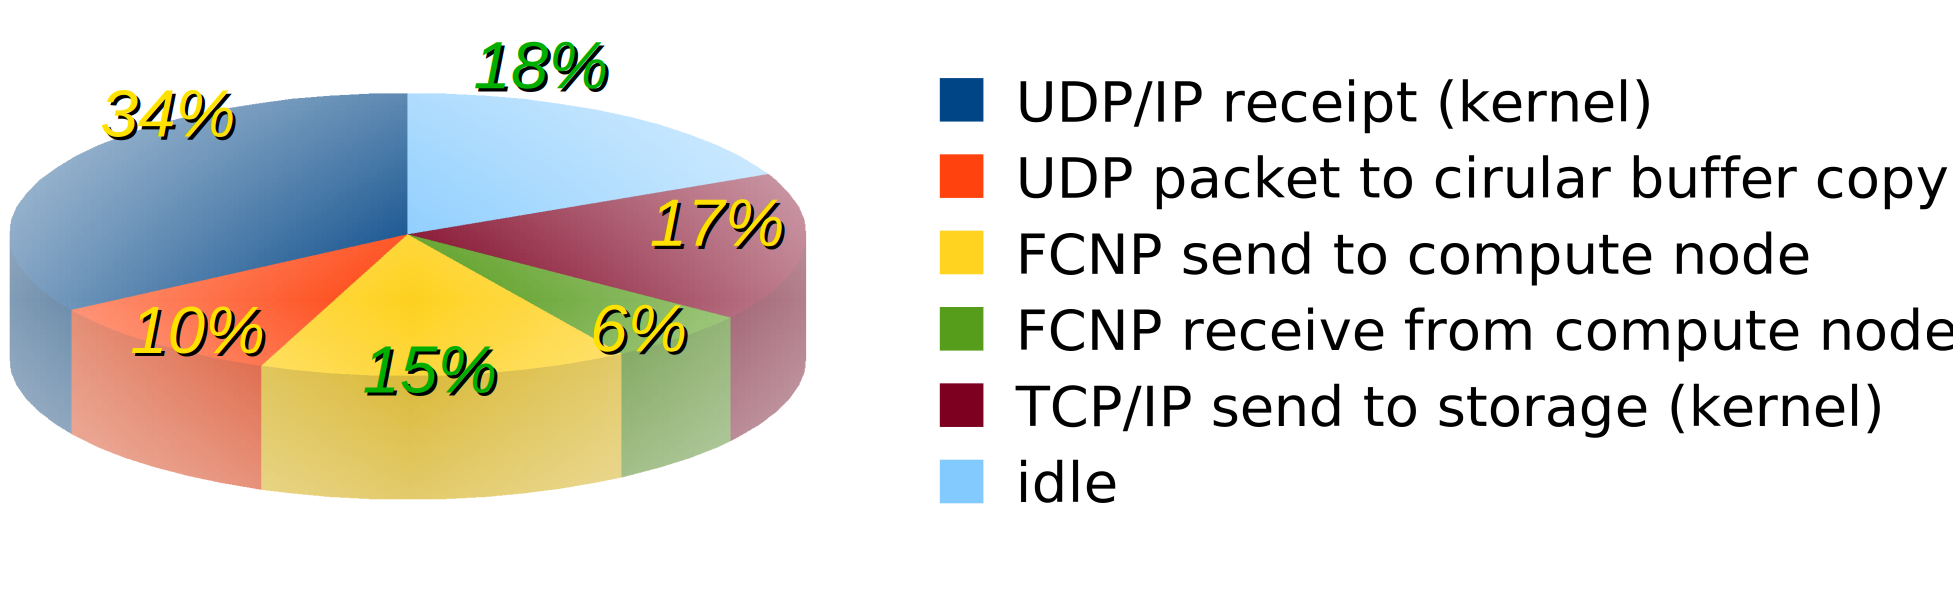
\includegraphics[width=\columnwidth]{ionode-load.pdf}
\caption{Performance breakdown on the I/O~node.}
\label{fig:ionode-load}
\end{figure}

We also measured how the LOFAR correlator benefits from FCNP.
Figure~\ref{fig:ionode-load} shows a breakdown of the processor
utilization on the I/O~node.
Apart from other tasks, each I/O~node sends 3.1~Gb/s and receives 1.2~Gb/s
from the compute nodes.
The data are sent directly from the circular buffer, without additional
copying (obeying the alignment restrictions, though, was rather complicated).
The Linux real-time scheduler (SCHED\_RR) runs both the sending and receiving
threads at the highest priority, to assure that the correlator can always
proceed.
These threads consume 15\% resp.\ 6\% of the total CPU power.
This is slightly more than the theoretical minimum of 12\% resp.\ 4.6\%,
mainly caused by the presence of other threads that compete for the same
resources (cache, memory, etcetera).
%The real-time scheduler runs the threads that send to and receive from the
%compute nodes at the highest priority, since these are essential to keep
%the correlator running at real time.
With a CPU utilization of 82\%, the I/O~node cannot handle much more without
starting dropping data.
Without FCNP, the required LOFAR data rates are not achieved;
with FCNP, the correlator runs smoothly over 50\% beyond the requirements.


\section{Conclusions}
\label{sec:conclusions}

This paper described \emph{Fast Collective Network Protocol (FCNP)}, a very
low-overhead network protocol for communication between the I/O~nodes and
compute nodes on the Blue Gene/P.
The relatively slow processor cores on this system are hardly capable to
keep up with the fast internal network, hence any protocol overhead
significantly slows down the obtained bandwidths.
Moreover, a low-overhead protocol is all the more important, because I/O~nodes
on the Blue Gene/P are much heavier loaded than I/O~nodes on its predecessor
Blue Gene/L.
To scale up, Blue Gene/P I/O~nodes must forward data 4.86~times faster than
Blue Gene/L I/O~nodes, over links that are only 2.43 faster, using processor
processor cores that are a marginal 21\% faster.

FCNP is critically important to the correlator of the LOFAR radio telescope.
One of the novel features of this telescope is that it does all real-time,
central processing in \emph{software\/} rather than hardware, but the
processing and bandwidth requirements demand the use of a supercomputer.
The standard system software is, however, not designed to provide user-level
bandwidths between I/O nodes and compute nodes at the required data rates.
FCNP, on the contrary, allows the LOFAR correlator to achieve bandwidths
that are even over 50\% beyond the requirements, keeping up with the
absolute maximum data rates that the LOFAR stations can produce.
As a consequence, a 50\% wider part of the spectrum can be observed
instantaneously, or alternatively, the number of concurrent observations
can be increased by a half.
Hence, with FCNP, the LOFAR telescope can be used much more efficiently than
it was ever designed for.




%6.6~Gb/s for future EoR observations.
%As supercomputers are usually not optimized for external I/O, streaming data
%into the correlator at these rates is challenging.
%One of the reasons to choose for the Blue Gene/L as correlator was its atypical
%high number of external GbE interfaces, 768 in six racks.

%Despite its potential, streaming data into the machine at the required rates
%turned out to be problematic~\cite{Romein:06}.
%Each GbE interface has to sustain at least 550~Mb/s in and 200~Mb/s out
%(concurrently) to keep up with the stations.
%Initially, the total bandwidth (in and out) obtained in practice peaked at
%about 300~Mb/s.
%After a year of updating drivers and tuning parameters, aggregate bandwidths
%of about 850~Mb/s were seen, provided that four (out of sixteen) compute nodes
%communicated concurrently through the same I/O~node, effectively wasting
%3/16$^\mathrm{rm}$ of all compute resources.
%Also, the higher data rates were only seen using benchmark programs; the
%application exhibits more complex communication patterns that had a
%devastating impact on the performance.


%Furthermore, there are improvements in reliability and power consumption.

%The improved programming environment and the change to 10-GbE technology
%had significant implications for our application.
%While the amount of FLOPS per rack has become 2.43 as high, the number of
%external interfaces has halved.
%As a consequence, each I/O~node has to handle (at least) four times as much
%data as on the BG/L.
%However, the total processing power on the BG/P has only improved by a factor
%of 2.43, while the load on the I/O~nodes of the BG/L was already problematic!
%Also, we measured that the link speed of the collective network that connects
%the I/O~node to the compute nodes cannot carry 6.54~Gb/s payload.
%Taking the high costs of the UDP/IP protocol stack into account, we thought
%that handling the full station data rate of 3.1~Gb % FIXME


\section*{Acknowledgments}

Chris Broekema, Jan David Mol, and Rob van Nieuwpoort made useful comments to
a draft version of this paper.
We thank Kamil Iskra and Kazutomo Yoshii from Argonne National Labs and 
Bruce Elmegreen, Todd Inglett, Tom Liebsch, and Andrew Tauferner from IBM for
their support.

LOFAR is funded by the Dutch government through the
BSIK program for interdisciplinary research and
improvement of the knowledge infrastructure. Additional
funding is provided through the European Regional
Development Fund and the innovation program
EZ/KOMPAS of the Collaboration of the Northern
Provinces (SNN). ASTRON is part of the Netherlands
Organization for Scientific Research, NWO.



\bibliographystyle{plain}
\bibliography{fcnp}

\end{document}
